\documentclass[11pt]{article}
\usepackage[margin=2.2cm,a4paper]{geometry}
\usepackage{booktabs,longtable,array,url,hyperref,graphicx,float}
% [H] pins each table where it is written. With nine floats and [h!], LaTeX moved
% tables away from the headings that introduce them.
\usepackage[T1]{fontenc}
\renewcommand{\arraystretch}{1.12}
% With every float pinned by [H], a page that is fractionally too full would otherwise
% be stretched past the bottom margin. Let pages end short instead.
\raggedbottom
% Each supplementary section starts a fresh page, so a heading is never separated from
% its table and no page ends with a large gap where a table would not fit.
\let\oldsection\section
\newcounter{supsec}
\renewcommand{\section}[1]{\stepcounter{supsec}\ifnum\value{supsec}>1\clearpage\fi\oldsection*{#1}}
\title{Supplementary Material\\\large The AI Incident Disclosure Shadow: Tracking AI Incidents into U.S. Securities Filings}
\author{Samir Chincholikar \and Robin Chawla}
\date{}
\begin{document}
\maketitle
\section*{Supplementary Material}
\setcounter{table}{0}\renewcommand{\thetable}{S\arabic{table}}
\renewcommand{\thefigure}{S\arabic{figure}}
% Only tables and figures carry S numbers. Numbering the sections as well produced two
% parallel S sequences, so that section S7 contained tables S8 and S9.
\setcounter{secnumdepth}{0}

\section{CSET AI-Harm severity for the externally classified subset}
Supplementary Table~S1 lists the 40 incidents carrying an external CSET AI-Harm classification,
unchanged from the original submission. For these incidents the CSET value was preserved rather than
assigned under the study rubric, and is reproduced verbatim from the released taxonomy.

{\scriptsize\renewcommand{\arraystretch}{1.0}
\begin{longtable}{@{}r p{8.6cm} l@{}}
\caption{The 40 incidents carrying an external CSET AI Harm Taxonomy classification, unchanged from the original submission. The remaining 267 incidents were assigned Severe, Moderate or Limited under the pre-specified study rubric and are not listed here.}\\
\toprule
AIID incident ID & CSET classification (harm level; tangible harm) & Study severity \\ \midrule
\endfirsthead
\toprule
AIID incident ID & CSET classification (harm level; tangible harm) & Study severity \\ \midrule
\endhead
\midrule \multicolumn{3}{r}{\emph{continued on next page}}\\
\endfoot
\bottomrule
\endlastfoot
81 & none; no tangible harm, near-miss, or issue & Moderate \\
82 & none; no tangible harm, near-miss, or issue & Moderate \\
83 & none; no tangible harm, near-miss, or issue & Moderate \\
84 & none; no tangible harm, near-miss, or issue & Moderate \\
89 & none; tangible harm definitively occurred & Severe \\
92 & AI tangible harm event; tangible harm definitively occurred & Severe \\
97 & AI tangible harm issue; non-imminent risk of tangible harm (an issue) occurred & Moderate \\
102 & none; no tangible harm, near-miss, or issue & Moderate \\
105 & AI tangible harm event; tangible harm definitively occurred & Severe \\
113 & none; no tangible harm, near-miss, or issue & Moderate \\
116 & AI tangible harm event; tangible harm definitively occurred & Severe \\
124 & AI tangible harm event; tangible harm definitively occurred & Severe \\
125 & AI tangible harm event; tangible harm definitively occurred & Severe \\
127 & none; tangible harm definitively occurred & Severe \\
129 & none; no tangible harm, near-miss, or issue & Moderate \\
139 & none; no tangible harm, near-miss, or issue & Moderate \\
142 & AI tangible harm issue; non-imminent risk of tangible harm (an issue) occurred & Moderate \\
143 & none; no tangible harm, near-miss, or issue & Moderate \\
144 & unclear; unclear & Limited \\
145 & AI tangible harm issue; non-imminent risk of tangible harm (an issue) occurred & Moderate \\
149 & AI tangible harm event; tangible harm definitively occurred & Severe \\
153 & AI tangible harm event; tangible harm definitively occurred & Severe \\
156 & none; tangible harm definitively occurred & Severe \\
157 & unclear; tangible harm definitively occurred & Severe \\
160 & AI tangible harm issue; non-imminent risk of tangible harm (an issue) occurred & Moderate \\
220 & AI tangible harm event; tangible harm definitively occurred & Severe \\
281 & none; non-imminent risk of tangible harm (an issue) occurred & Moderate \\
313 & none; no tangible harm, near-miss, or issue & Moderate \\
354 & AI tangible harm event; tangible harm definitively occurred & Severe \\
360 & none; no tangible harm, near-miss, or issue & Moderate \\
367 & none; no tangible harm, near-miss, or issue & Moderate \\
393 & none; no tangible harm, near-miss, or issue & Moderate \\
414 & none; no tangible harm, near-miss, or issue & Moderate \\
489 & none; no tangible harm, near-miss, or issue & Moderate \\
501 & AI tangible harm event; tangible harm definitively occurred & Severe \\
554 & none; no tangible harm, near-miss, or issue & Moderate \\
574 & none; no tangible harm, near-miss, or issue & Moderate \\
576 & none; no tangible harm, near-miss, or issue & Moderate \\
583 & none; no tangible harm, near-miss, or issue & Moderate \\
614 & none; no tangible harm, near-miss, or issue & Moderate \\
\end{longtable}}

\section{T3 coding examples}
The T3 threshold requires filing language that names the \emph{class} of technology or the
\emph{class} of harm implicated in the incident. The examples below are drawn from the per-incident
filing-search records in the replication package. Positive examples qualified as T3a, where the
filing language matched both the incident's technology family and its harm family; negative examples
qualified only as T3b, where a single family matched, which is the distinction this split isolates.
Fragments are quoted verbatim from the coding record and truncated to at most forty words.

\begin{table}[H]
\caption{Worked T3 coding examples, one T3a and one T3b per domain, each incident used once. \emph{Qualified} reports which of the incident's two families the filing language matched: a T3a example matched both, a T3b example only one, which is why a T3b case does not support the reading that the generic language is closely related to the realized incident. Fragments are quoted verbatim from the filing-search record and truncated.}
\centering\scriptsize
\begin{center}
\begin{tabular}{@{}p{1.9cm}cr p{1.7cm} p{2.5cm} p{4.6cm}@{}}
\toprule
Domain & Split & AIID id & Issuer & Qualified (app / harm) & Verbatim fragment from the filing record \\ \midrule
content / misinformation & T3a & 1302 & Alphabet & generative-llm / misinformation-content & harmful content ... violation of rights of publicity, defamation \\
content / misinformation & T3b & 84 & Meta & --- / misinformation-content & negative publicity in connection with our handling of misinformation... including in connection with the COVID-19 pandemic and elections \\
generative-AI error & T3a & 674 & Alphabet & generative-llm / misinformation-content & harmful content ... may create new avenues of abuse for bad actors \\
generative-AI error & T3b & 467 & Alphabet & generative-llm / --- & Our evolving AI-related efforts may give rise to risks related to harmful content, inaccuracies... and other issues. \\
autonomous system & T3a & 181 & GM & autonomous-vehicle / physical-safety & Our AV strategy is dependent upon our ability to successfully mitigate unique technological, operational and regulatory risks... To the extent accidents... associated with our autonomous driving systems occur, we could be subject to liability, \\
autonomous system & T3b & 540 & Tesla & autonomous-vehicle / --- & misuse or claimed failures... of such new technologies \\
bias / discrimination & T3a & 161 & Meta & ads-targeting / discrimination-bias & changes reduce our ability to effectively target ads... adversely affected our advertising business \\
bias / discrimination & T3b & 645 & Alphabet & --- / discrimination-bias & Issues in the development and use of AI may result in reputational harm. \\
\bottomrule
\end{tabular}
\end{center}
\end{table}

\section{Entity resolution detail}
\begin{table}[H]
\caption{Incidents in the analytical sample with more than one listed-issuer candidate. The original procedure retained one issuer per incident, selected by listing status with ties broken by the order of organizations in the AIID record; the discarded candidates were not persisted and are re-derived here.}
\centering\scriptsize
\begin{tabular}{@{}rlp{4.2cm}p{5.4cm}@{}}
\toprule
AIID id & Date & Issuer retained & Listed candidates discarded \\ \midrule
83 & 2020-10-22 & Microsoft Corporation & Alphabet Inc. \\
92 & 2019-11-11 & The Goldman Sachs Group Inc. & Apple Inc. \\
102 & 2020-03-23 & Microsoft Corporation & Alphabet Inc.; Amazon.com, Inc.; Apple Inc.; International Business Machines \\
168 & 2022-03-01 & Meta Platforms, Inc. & Alphabet Inc.; Microsoft Corporation; Netflix, Inc.; Twitter, Inc. \\
143 & 2021-02-16 & Meta Platforms, Inc. & Twitter, Inc. \\
268 & 2020-03-16 & Meta Platforms, Inc. & Alphabet Inc.; Twitter, Inc. \\
343 & 2021-07-11 & Meta Platforms, Inc. & Twitter, Inc. \\
359 & 2021-05-23 & Meta Platforms, Inc. & Twitter, Inc. \\
475 & 2021-06-02 & McDonald's Corporation & International Business Machines \\
587 & 2023-05-22 & Alphabet Inc. & Amazon.com, Inc.; Apple Inc.; Microsoft Corporation \\
718 & 2024-04-06 & Meta Platforms, Inc. & Alphabet Inc. \\
731 & 2023-12-01 & Meta Platforms, Inc. & Alphabet Inc. \\
734 & 2024-06-18 & Microsoft Corporation & Alphabet Inc.; Meta Platforms, Inc. \\
744 & 2024-06-25 & Microsoft Corporation & Alphabet Inc. \\
750 & 2024-07-22 & Meta Platforms, Inc. & Alphabet Inc. \\
846 & 2021-10-06 & Meta Platforms, Inc. & X Corp. (fmr Twitter) \\
859 & 2024-10-30 & Alphabet Inc. & Meta Platforms, Inc. \\
881 & 2024-12-27 & Serve Robotics Inc. & Alphabet Inc. \\
967 & 2025-03-06 & Alphabet Inc. & Amazon.com, Inc. \\
968 & 2022-02-24 & Microsoft Corporation & Alphabet Inc.; Meta Platforms, Inc. \\
1186 & 2025-07-31 & Microsoft Corporation & Alibaba Group Holding \\
1188 & 2025-06-25 & Microsoft Corporation & Alphabet Inc. \\
1210 & 2025-08-21 & Alphabet Inc. & Amazon.com, Inc. \\
1279 & 2025-11-18 & Microsoft Corporation & Alphabet Inc.; Meta Platforms, Inc. \\
1436 & 2022-06-23 & Integra LifeSciences Holdings & Johnson \& Johnson \\
1528 & 2023-05-19 & Integra LifeSciences Holdings & Johnson \& Johnson \\
1575 & 2026-01-20 & PayPal Holdings, Inc. & Microsoft Corporation \\
\bottomrule
\end{tabular}
\end{table}

\begin{table}[H]
\caption{Stage-by-stage exclusion accounting. Of 1{,}389 window incidents, 1{,}082 are excluded and 307 remain. Note that foreign private issuers and delisted issuers are excluded \emph{after} a successful organization-to-registrant match, which is why the mapped file contains 348 rows (307 + 26 + 15).}
\centering\small
\begin{tabular}{@{}p{3.0cm}p{4.6cm}rp{4.9cm}@{}}
\toprule
Stage & Exclusion & n & Sub-reason \\ \midrule
1. Date window & outside 2019--2026 & 208 & of 1{,}597 snapshot records \\ \midrule
2. Organization named & generic or individual actors only & 398 & scammers, users, unnamed developers, government bodies \\
3. Organization resolvable & named entity not in the crosswalk & 400 & unresolved corporate or institutional names \\
4. Listed status & privately held & 243 & dominated by private AI labs \\ \midrule
5. Post-match: domicile & foreign private issuer (20-F/6-K) & 26 & Baidu, Alibaba, Thomson Reuters and others \\
6. Post-match: listing & excluded under the study's delisted-issuer rule & 15 & Twitter/X Corp., Rite Aid \\ \midrule
\multicolumn{2}{@{}l}{\textbf{Total excluded}} & \textbf{1{,}082} & \\
\multicolumn{2}{@{}l}{\textbf{Analytical sample}} & \textbf{307} & 21 issuers \\
\bottomrule
\end{tabular}
\end{table}

\section{Severity}
\begin{table}[H]
\caption{Tier distribution for the 40 incidents carrying an external CSET AI-Harm severity classification. The subset contains 1 substantive disclosure, so no inferential test is performed (fewer than 5 substantive cases).}
\centering\small
\begin{tabular}{@{}lrrrrr@{}}
\toprule
CSET severity & n & T1 & T2 & T3a & T3b \& T4 \\ \midrule
severe & 14 & 1 & 0 & 3 & 10 \\
moderate & 25 & 0 & 0 & 7 & 18 \\
limited & 1 & 0 & 0 & 1 & 0 \\
\bottomrule
\end{tabular}
\end{table}

\section{Role analysis fragility}
\begin{table}[H]
\caption{Leave-one-positive-out sensitivity of the role association. Each of the seven substantive incidents is in turn dropped, reclassified one tier down, and reclassified to T3; both contrasts are recomputed by Monte-Carlo exact permutation (20{,}000 draws, seed 42). The final row promotes one developer-only T3 incident to T1 as an upper-bound perturbation.}
\centering\small
\begin{tabular}{@{}llrrrr@{}}
\toprule
Perturbation & Incident & \multicolumn{2}{c}{3-way contrast} & \multicolumn{2}{c}{2$\times$2 contrast} \\
 & & $\chi^2$ & $p$ & $\chi^2$ & $p$ \\ \midrule
none (baseline, adjudicated) & - & 10.434 & 0.0242 & 1.669 & 0.3552 \\
drop & 149 & 3.416 & 0.2191 & 1.431 & 0.3634 \\
one tier down & 149 & 10.434 & 0.0242 & 1.669 & 0.3552 \\
reclassify to T3 & 149 & 3.16 & 0.2236 & 1.425 & 0.3650 \\
drop & 534 & 12.3 & 0.0170 & 1.431 & 0.3709 \\
one tier down & 534 & 12.344 & 0.0172 & 1.425 & 0.3649 \\
reclassify to T3 & 534 & 12.344 & 0.0172 & 1.425 & 0.3649 \\
drop & 596 & 12.3 & 0.0187 & 1.431 & 0.3676 \\
one tier down & 596 & 10.434 & 0.0242 & 1.669 & 0.3552 \\
reclassify to T3 & 596 & 12.344 & 0.0162 & 1.425 & 0.3628 \\
drop & 711 & 12.3 & 0.0189 & 1.431 & 0.3677 \\
one tier down & 711 & 12.344 & 0.0176 & 1.425 & 0.3631 \\
reclassify to T3 & 711 & 12.344 & 0.0176 & 1.425 & 0.3631 \\
drop & 726 & 12.3 & 0.0191 & 1.431 & 0.3688 \\
one tier down & 726 & 10.434 & 0.0242 & 1.669 & 0.3552 \\
reclassify to T3 & 726 & 12.344 & 0.0174 & 1.425 & 0.3680 \\
drop & 733 & 3.416 & 0.2194 & 1.431 & 0.3651 \\
one tier down & 733 & 10.434 & 0.0242 & 1.669 & 0.3552 \\
reclassify to T3 & 733 & 3.16 & 0.2248 & 1.425 & 0.3650 \\
drop & 997 & 12.3 & 0.0176 & 1.431 & 0.3602 \\
one tier down & 997 & 10.434 & 0.0242 & 1.669 & 0.3552 \\
reclassify to T3 & 997 & 12.344 & 0.0179 & 1.425 & 0.3665 \\
promote one developer-only T3 incident to T1 & 81 & 7.915 & 0.0537 & 0.219 & 0.7079 \\
\bottomrule
\end{tabular}
\end{table}

\section{Reliability by tier}
\begin{table}[H]
\caption{One-tier-against-the-rest agreement in the stratified reliability sample (n = 68), and the full confusion matrix. The T2 coefficient is negative: the second coder assigned the three pass-one T2 incidents to T1, T3 and T4 respectively, agreeing with none. T2 therefore has no demonstrated inter-coder reliability in this sample, which is why T1 is the primary measure of incident-specific disclosure and T1+T2 is reported as an upper bound.}
\centering\small
\begin{tabular}{@{}lrrr@{}}
\toprule
Tier & n (pass 1) & Raw agreement & Cohen's $\kappa$ \\ \midrule
T1 & 4 & 0.971 & 0.734 \\
T2 & 3 & 0.941 & -0.023 \\
T3 & 40 & 0.882 & 0.755 \\
T4 & 21 & 0.912 & 0.793 \\
\midrule
\multicolumn{4}{@{}l}{Aggregate: raw 0.853, $\kappa$ 0.726, PABAK 0.706, Gwet AC1 0.821 } \\
\bottomrule
\end{tabular}

\vspace{4pt}
\begin{tabular}{@{}lrrrr@{}}
\toprule
Pass 1 $\downarrow$ / Pass 2 $\rightarrow$ & T1 & T2 & T3 & T4 \\ \midrule
T1 & 3 & 0 & 1 & 0 \\
T2 & 1 & 0 & 1 & 1 \\
T3 & 0 & 1 & 37 & 2 \\
T4 & 0 & 0 & 3 & 18 \\
\bottomrule
\end{tabular}
\end{table}

\section{Reliability of issuer matching}
\begin{table}[H]
\caption{Agreement on issuer identity between the study mapping and a blind second coder, by sampling stratum. The sample of 80 incidents (seed 42) deliberately oversamples ambiguous cases, so the overall rate is expected to be conservative relative to full-sample agreement. Overall: 82.5\% raw agreement, Cohen's $\kappa$ = 0.79, Gwet's AC1 = 0.82. Post-hoc; not pre-specified.}
\label{tab:entrel}
\centering\small
\begin{tabular}{@{}lrrr@{}}
\toprule
Stratum & n & Agree & Agreement \\ \midrule
Mapped through a subsidiary or product & 30 & 30 & 100.0\% \\
More than one listed candidate & 27 & 13 & 48.1\% \\
Issuer contributing three or fewer incidents & 13 & 13 & 100.0\% \\
Single candidate, frequent issuer & 10 & 10 & 100.0\% \\
\midrule
\emph{Second coder's own confidence: high} & 47 & 47 & 100.0\% \\
\emph{Second coder's own confidence: low} & 18 & 11 & 61.1\% \\
\emph{Second coder's own confidence: medium} & 15 & 8 & 53.3\% \\
\bottomrule
\end{tabular}
\end{table}

\begin{table}[H]
\caption{Every disagreement on issuer identity, with its adjudication against the attribution rules of Section~3.2. Ten resolve in favour of the study mapping, four in favour of the second coder. None involves an incident coded T1 or T2. Post-hoc; not pre-specified.}
\label{tab:entadj}
\centering\footnotesize
\begin{tabular}{@{}llll@{}}
\toprule
Incident & Study mapping & Second coder & Adjudication \\ \midrule
102 & Microsoft & Apple & study stands \\
168 & Meta & Netflix, Inc. & study stands \\
268 & Meta & Alphabet & study stands \\
475 & McDonald's Corporation & International Business Machines & study stands \\
587 & Alphabet & Apple & study stands \\
718 & Meta & NONE-not-listed & study stands \\
731 & Meta & Alphabet & study stands \\
750 & Meta & Alphabet & study stands \\
846 & Meta & Twitter, Inc. & study stands with qualification \\
881 & Serve Robotics & Alphabet & second coder \\
967 & Alphabet & Amazon & study stands with qualification \\
1436 & Integra LifeSciences Holdings & Johnson \& Johnson & second coder \\
1528 & Integra LifeSciences Holdings & Johnson \& Johnson & second coder \\
1575 & PayPal Holdings, Inc. & NONE-not-listed & second coder on basis \\
\bottomrule
\end{tabular}
\end{table}

\section{Shadow rate by severity}
\begin{figure}[H]
\centering
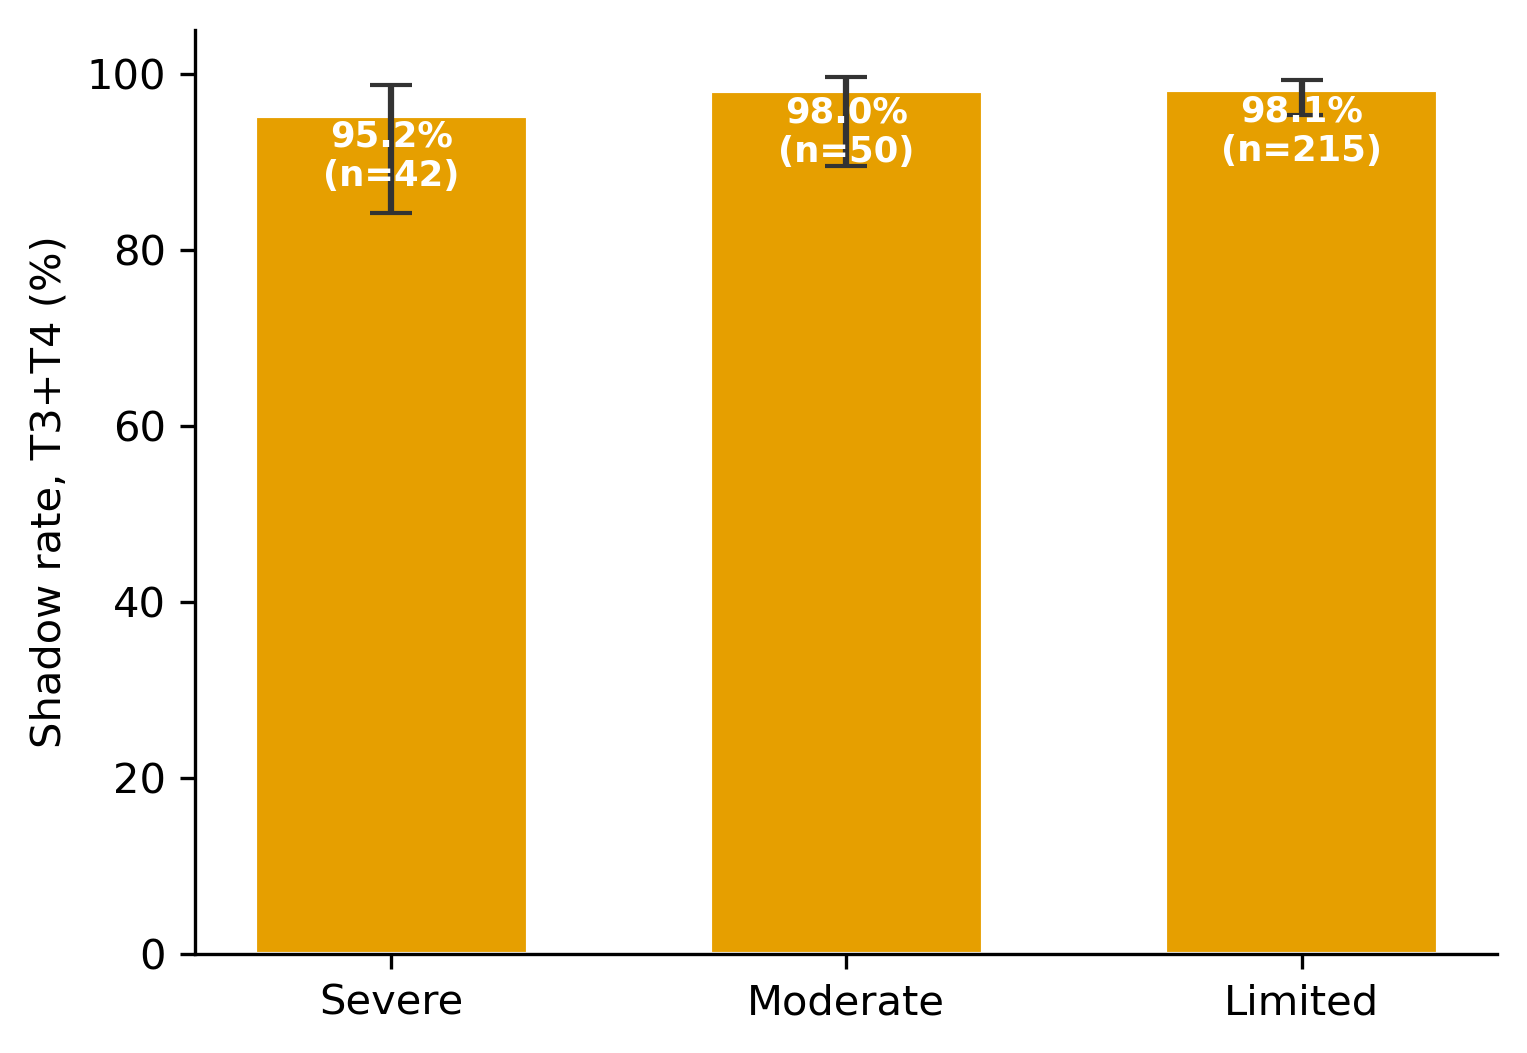
\includegraphics[width=0.78\textwidth]{FigureS1.png}
\caption{Collapsed shadow rate (T3+T4) by incident severity, with 95\% Wilson intervals. Figure~2 of the main text gives the same strata as a five-way distribution across all tiers.}
\label{fig:supp-sev}
\end{figure}
\end{document}
